\documentclass[portuguese, conference]{IEEEtran}
\usepackage{blindtext, graphicx}
\usepackage[]{algorithm2e}
\usepackage[T1]{fontenc}
\usepackage[utf8]{inputenc}
\graphicspath{{images/}}

\ifCLASSINFOpdf
\else
\fi

% correct bad hyphenation here
\hyphenation{op-tical net-works semi-conduc-tor}

\begin{document}
\title{Programação Paralela: Paradigma Pipeline}

% author names and affiliations
% use a multiple column layout for up to three different
% affiliations
\author{\IEEEauthorblockN{Filipe Franciel Utzig}
\IEEEauthorblockA{Engenharia de Computação\\
Pontifícia Universidade Católica do Rio Grande do Sul - PUCRS\\
Porto Alegre 90619-900
\\
Email: filipeutzig \textit{at} gmail.com}}

% make the title area
\maketitle

\begin{abstract}
\it{The present work presents the implementation of sorting algorithm known as Insertion Sort, this algorithm will be presented in two forms: parallel, using openMPI library with the pipeline paradigm, and sequential, so that, at the end, we can have a better knowledge regarding the performance and efficiency of the parallel version.}
\end{abstract}

% Note that keywords are not normally used for peerreview papers.
\begin{IEEEkeywords}
MPI; Insertion-Sort; parallelism; pipeline; performance;
\end{IEEEkeywords}

\IEEEpeerreviewmaketitle

\section{Introdução}
No cenário computacional atual o uso de sistemas multi-processados é algo comum, mesmo entre sistemas embarcados como \textit{smartphones}. Neste contexto explorar o uso de programação paralela torna-se muito interessante. Entre as diversas técnicas de programação paralela existentes, neste trabalho, será explorado o paradigma de pipeline sobre o problema o problema de ordenação de dados, utilizando o \textit{Insertion Sort}.

Este algoritmo funciona construindo o vetor ordenado de um item por vez, ao receber um valor \textit{x}, ele é comparado a cada um dos valores já posicionados no vetor de saída, de forma a verificar qual a posição em que \textit{x} deve ser inserido. Feita a inserção, o algoritmo deve agora recolocar todos os elementos seguintes uma posição adiante. O processo se repete para \textit{x+1, x+2, etc…} até que todo o vetor esteja ordenado. O Insertion Sort, ao contrário de outros algoritmos, passa através do vetor uma só vez. Esse algoritmo, também é comumente comparado à organizar, de maneira crescente, as cartas de um baralho.~\cite{Insertion}.

\section{Detalhamento do problema}

A rotina de funcionamento acima mencionada pode ser visualizada no Algoritmo (\ref{Insertion_Sort}).

\begin{algorithm}[ht]
\label{Insertion_Sort}
    \For{(i = 0; i < n; i++)} {
        val = unsorted[i]\;
        \For{(j = 0; j < i; j++)} {
            \If{(val < sorted[j]} {
                aux = sorted[j]\;
                sorted[j] = val\;
                val = aux\;
            }
        }
        sorted[i] = val\;
    }
\caption{{\it Insertion Sort}}
\end{algorithm}

Para implementar o algoritmo~\ref{Insertion_Sort} foi utilizado a linguagem programação C e, na versão paralela deste, a biblioteca openMPI~\cite{HAM13}, rodando sobre o sistema operacional Linux.

\subsection{Detalhamento da versão sequencial}
A versão sequencial do algoritmo segue o mesmo principio de funcionamento da versão paralela, que será apresentada a seguir, porém seu desenvolvimento é simplificado quando comparado a versão paralela. O algoritmo utiliza dois vetores para realizar o ordenamento: O primeiro contém os valores desordenados e o segundo vetor é serão armazenados os valores ordenados.

Para cada elemento {\it x} retirado do vetor desordenado, o algoritmo percorre o vetor ordenado até achar um elemento {\it y} tal que ({\it x < y}). Ao encontrar este elemento, seu valor é armazenado em uma variável auxiliar e {\it x} é inserido na posição em que estava {\it y}. O algoritmo repete os passos acima, desta vez para o elemento {\it y}. O processo se repete até que não haja mais elementos no vetor desordenado. Caso não encontre, no vetor ordenado, nenhum elemento {\it y} que satisfaça a condição ({\it x < y}), ele simplesmente adiciona o valor {\it x} no final do vetor ordenado, visto que {\it x} é o maior elemento deste vetor.

\subsection{Detalhamento da versão paralela}
A versão paralela funciona da seguinte maneira: Cada processo possui um vetor com tamanho definido por \textbf{n/P} onde \textbf{n} é o número total de elementos a serem ordenados, e \textbf{P} é o número de processos utilizados. O primeiro estágio do {\it pipeline} tem um funcionamento levemente diferente dos outros, é o primeiro estágio que contém o vetor de entrada armazenado em memória. O primeiro estágio inicia a inserção ordenada na sua fatia do vetor resultado, quando a fatia do vetor resultado do primeiro estágio estiver cheio, a inserção de um valor resulta na saída de outro, o valor removido é então enviado para o próximo estágio do {\it pipeline}, este processo de inserção é repetido até que não tenha haja mais nenhum valor para ser ordenado. 

O processo acaba assim que o último estágio terminar de ordenar o seu vetor, neste momento é feita a tomada de tempo para avaliação dos resultados.

\section{Resultados}
Todos os testes foram executados no {\it cluster} Atlântica que é composto por 16 máquinas Dell PowerEdge R610. Cada máquina possui dois processadores Intel Xeon Quad-Core E5520 2.27 GHz Hyper-Threading e 16GB de memória, totalizando 8 núcleos (16 threads) por nó e 128 núcleos (256 threads) no custer. Os nós estão interligadas por 4 redes Gigabit-Ethernet chaveadas. O ultimo nó (atlantica16), dispõe de uma NVIDIA Tesla S2050 Computing System, com 4 NVIDIA Fermi computing processors (448 CUDA cores cada) divididos em 2 host interfaces e 12GB de memória.~\cite{IDE15}

A Tabela~\ref{tab1} contém os tempos de execução dos testes, cada teste foi executado 29 vezes a fim de aumentar a confiabilidade dos dados adquiridos, para isso foi desenvolvido um {\it script} de forma a automatizar a execução  e criar uma relação de todos os tempos obtidos, após esse processo a média de todas as execuções foi calculada. Podemos observar um decréscimo de tempo em todos os casos com a paralelização dos processos, esse comportamento ocorre pois cada estágio do pipeline ordena uma fatia menor, não percorrendo toda a extensão do vetor. Podemos observar melhor esse comportamento através da Figura ~\ref{fig:tempo}.

\begin{figure}[htb]
\raggedright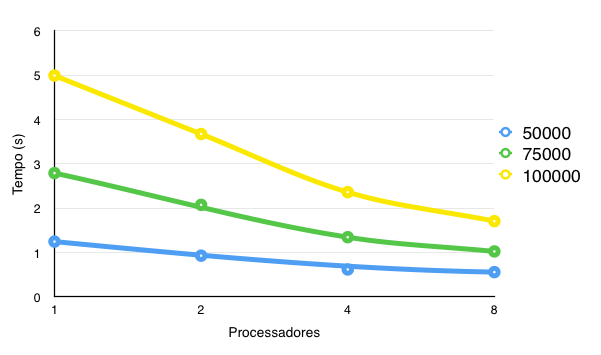
\includegraphics[width=.5\textwidth]{tempo.png}
\caption{\label{fig:tempo}Tempo de Execução.}
\end{figure}

\begin{table}[h]
\centering
\caption{Tempo de execução dos testes.}
\label{tab1}
\begin{tabular}{|c|l|l|l|}
\hline
\multicolumn{1}{|l|}{\begin{tabular}[c]{@{}l@{}}Número de\\ Processadores\end{tabular}} & \begin{tabular}[c]{@{}l@{}}50000 \\ Elementos\end{tabular} & \begin{tabular}[c]{@{}l@{}}75000 \\ Elementos\end{tabular} & \begin{tabular}[c]{@{}l@{}}100000\\ Elementos\end{tabular} \\ \hline
1           & 1,245             & 2,791             & 4,992        \\ \hline
2           & 0,927             & 2,074             & 3,673        \\ \hline
4           & 0,616             & 1,344             & 2,361        \\ \hline
8           & 0,556             & 1,023             & 1,707        \\ \hline
\end{tabular}
\end{table}

O aumento de velocidade foi observado nos estudos de caso, para quantificar o tempo de resposta de cada caso, foi calculado o {\it Speed Up} de cada cenário de teste, que é obtido de acordo com a Equação (\ref{eq:eq1}) onde T\textsubscript{s} é o tempo do programa sequencial e T{\textsubscript{n}} é o tempo do programa paralelo, a Tabela~\ref{speed_up} contém todos os valores referentes a {\it Speed Up}, nela podemos observar que neste caso o desempenho possui um comportamento linear para os cenários de teste analisados. 

Analisando os resultados é possível verificar uma diminuição no crescimento do valor de {\it Speed Up} a partir de 8 processadores com 50000 elementos, este comportamento é justificado pois o número de elementos processados por cada estágio do pipeline diminuí bastante e o {\it overhead} de comunicação passa a ser mais perceptível. Podemos observar comportamento das avaliações de {\it Speed Up} através da Figura~\ref{fig:speed}.

\begin{equation}\label{eq:eq1}
    Speed Up = \frac{T\textsubscript{s}}{ T\textsubscript{n}}
\end{equation}

\begin{table}[h]
\centering
\caption{Speed Up}
\label{speed_up}
\begin{tabular}{|c|c|c|c|}
\hline
\begin{tabular}[c]{@{}c@{}}Número de\\ Processadores\end{tabular} & \begin{tabular}[c]{@{}c@{}}50000 \\ Elementos\end{tabular} & \begin{tabular}[c]{@{}c@{}}75000 \\ Elementos\end{tabular} & \begin{tabular}[c]{@{}c@{}}100000 \\ Elementos\end{tabular} \\ \hline
1           & 1                 & 1                 & 1             \\ \hline
2           & 1,34              & 1,35              & 1,36          \\ \hline
4           & 2,02              & 2,08              & 2,11          \\ \hline
8           & 2,24              & 2,73              & 2,92          \\ \hline
\end{tabular}
\end{table}

\begin{figure}[htb]
\raggedright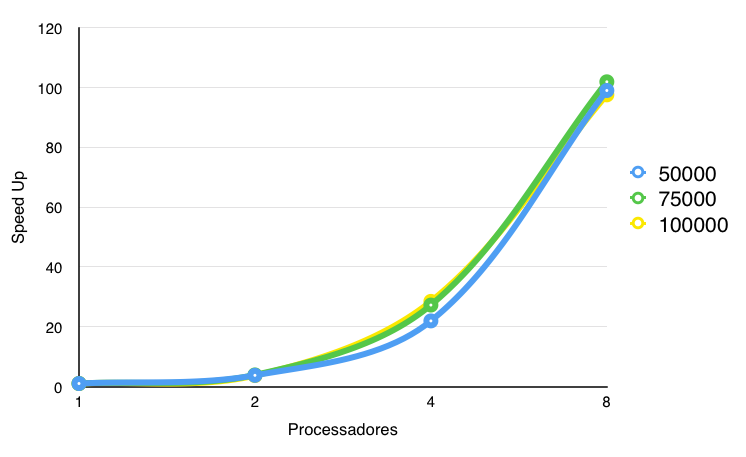
\includegraphics[width=.5\textwidth]{speedup.png}
\caption{\label{fig:speed}Speed up.}
\end{figure}

A eficiência com a paralelização também foi calculada e é obtida através da Equação (~\ref{eq:eq2}), todos os dados encontram-se na Tabela~\ref{efic}. Observamos que ocorre uma redução no ganho de eficiência do programa ao aumentarmos o número de processadores, isto é, ao aumentarmos em {\it n} vezes os processadores usados, o desempenho não aumentará na mesma proporção, já que a otimização do algoritmo ao aumentar o paralelismo não é linear.

O comportamento da eficiência dessa paralelização está ilustrada na Figura~\ref{fig:eficiencia}.

\begin{table}[h]
\centering
\caption{Eficiência dos testes.}
\label{efic}
\begin{tabular}{|c|c|c|c|}
\hline
\begin{tabular}[c]{@{}c@{}}Número de\\ Processadores\end{tabular} & \begin{tabular}[c]{@{}c@{}}50000 \\ Elementos\end{tabular} & \begin{tabular}[c]{@{}c@{}}75000 \\ Elementos\end{tabular} & \begin{tabular}[c]{@{}c@{}}100000 \\ Elementos\end{tabular} \\ \hline
1           & 1                 & 1                 & 1             \\ \hline
2           & 0,67              & 0,67              & 0,68          \\ \hline
4           & 0,51              & 0,52              & 0,53          \\ \hline
8           & 0,28              & 0,34              & 0,37          \\ \hline
\end{tabular}
\end{table}
\begin{equation}\label{eq:eq2}
    Eficiencia = \frac{SpeedUp}{n}
\end{equation}

\begin{figure}[htb]
\raggedright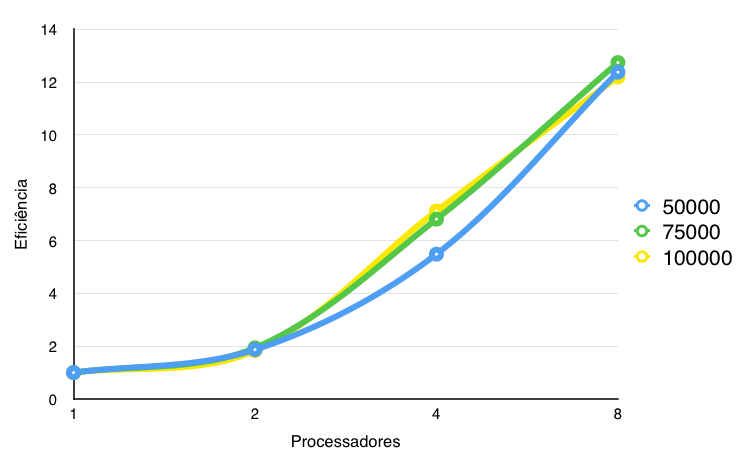
\includegraphics[width=.5\textwidth]{eficiencia.png}
\caption{\label{fig:eficiencia}Eficiência.}
\end{figure}

\section{Conclusão}

Podemos observar que com a paralelização do problema obtivemos um ganho de desempenho significativo. Nos cenários simulados foi possível verificar que conforme o número de processadores foi aumentando o {\it Speed Up} também aumentava, porém esse comportamento não é linear, pois se aumentarmos muito o número de processadores chegaremos um ponto em que o gargalo será a comunicação entre esses diversos processos, comportamento este que começou a ser observado com o uso de 8 processadores e um número menor de elementos processados.

\bibliographystyle{IEEEtranS}
\bibliography{referencia}

\end{document}
